\documentclass[border=6pt]{standalone}
\usepackage{tikz}
\usetikzlibrary{arrows.meta,calc,decorations.pathreplacing,positioning}
\begin{document}

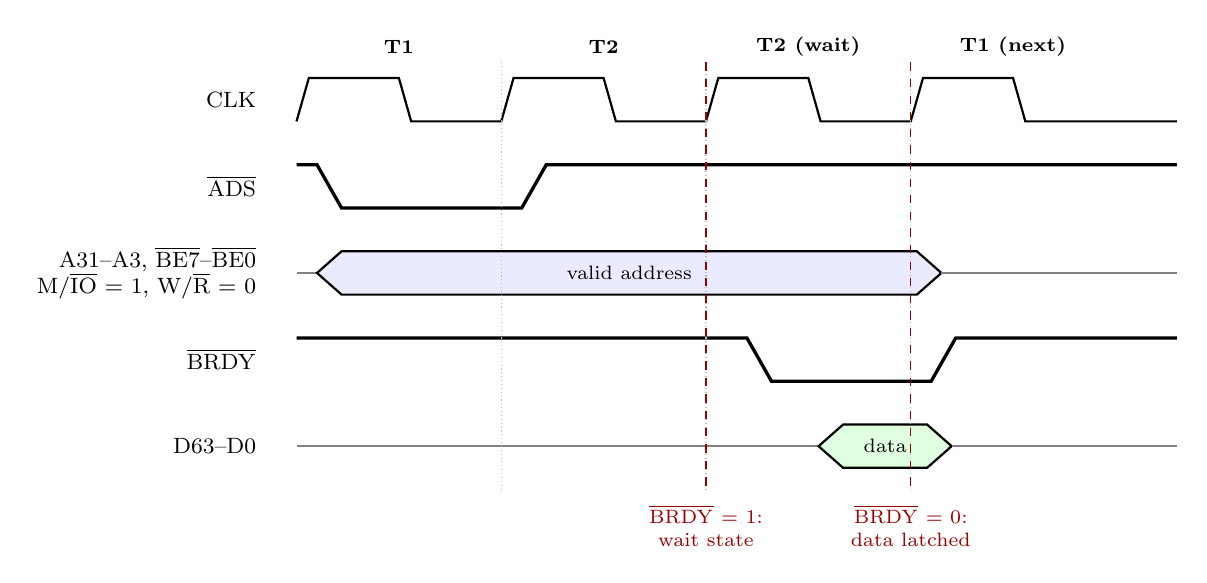
\begin{tikzpicture}[>=Stealth,font=\small,x=2.6cm,y=1cm]
% row 0 y=0
\node[anchor=east,font=\footnotesize,align=right] at (-0.15,0.275) {CLK};
\draw[thick] (0,0) -- (0,0) -- (0.06,0.55) -- (0.5,0.55) -- (0.56,0) -- (1,0) -- (1.06,0.55) -- (1.5,0.55) -- (1.56,0) -- (2,0) -- (2.06,0.55) -- (2.5,0.55) -- (2.56,0) -- (3,0) -- (3.06,0.55) -- (3.5,0.55) -- (3.56,0) -- (4.3,0);
% row 1 y=-1.1
\node[anchor=east,font=\footnotesize,align=right] at (-0.15,-0.825) {$\overline{\mathrm{ADS}}$};
\draw[very thick] (0,-0.55) -- (0.1,-0.55) -- (0.22,-1.1) -- (1.1,-1.1) -- (1.22,-0.55) -- (4.3,-0.55);
% row 2 y=-2.2
\node[anchor=east,font=\footnotesize,align=right] at (-0.15,-1.925) {A31--A3, $\overline{\mathrm{BE7}}$--$\overline{\mathrm{BE0}}$\\M/$\overline{\mathrm{IO}}$ = 1, W/$\overline{\mathrm{R}}$ = 0};
\draw[thick,gray] (0,-1.925) -- (0.1,-1.925);
\draw[thick,fill=blue!8] (0.1,-1.925) -- (0.22,-1.65) -- (3.03,-1.65) -- (3.15,-1.925) -- (3.03,-2.2) -- (0.22,-2.2) -- cycle;
\node[font=\scriptsize] at (1.625,-1.925) {valid address};
\draw[thick,gray] (3.15,-1.925) -- (4.3,-1.925);
% row 3 y=-3.3
\node[anchor=east,font=\footnotesize,align=right] at (-0.15,-3.025) {$\overline{\mathrm{BRDY}}$};
\draw[very thick] (0,-2.75) -- (2.2,-2.75) -- (2.32,-3.3) -- (3.1,-3.3) -- (3.22,-2.75) -- (4.3,-2.75);
% row 4 y=-4.4
\node[anchor=east,font=\footnotesize,align=right] at (-0.15,-4.125) {D63--D0};
\draw[thick,gray] (0,-4.125) -- (2.55,-4.125);
\draw[thick,fill=green!12] (2.55,-4.125) -- (2.67,-3.85) -- (3.08,-3.85) -- (3.2,-4.125) -- (3.08,-4.4) -- (2.67,-4.4) -- cycle;
\node[font=\scriptsize] at (2.875,-4.125) {data};
\draw[thick,gray] (3.2,-4.125) -- (4.3,-4.125);

\foreach \x/\l in {0.5/T1,1.5/T2,2.5/T2 (wait),3.5/T1 (next)} \node[font=\scriptsize\bfseries] at (\x,0.95) {\l};
\foreach \t in {1,2,3} \draw[gray!50,densely dotted] (\t,0.75) -- (\t,-4.7);
\draw[red!60!black,dashed] (2,0.75) -- (2,-4.7);
\draw[red!60!black,dashed] (3,0.75) -- (3,-4.7);
\node[font=\scriptsize,red!60!black,align=center,anchor=north] at (2,-4.75) {$\overline{\mathrm{BRDY}}$ = 1:\\wait state};
\node[font=\scriptsize,red!60!black,align=center,anchor=north] at (3,-4.75) {$\overline{\mathrm{BRDY}}$ = 0:\\data latched};

\end{tikzpicture}
\end{document}
